\chapter{Introduction}
\label{chap:intro}

\section{Networks and systems pervade}
Different types of networks play a critical role in our every day lives. We use Public Switched Telephone Networks (PSTN) and cellular networks to communicate with people by making voice calls (and sending text messages in case of cellular networks). PSTN and cellular networks also server as access media for connecting to the Internet, which offers several key services. We communicate and collaborate using email, voice/video calls over Internet Protocol (IP) and social networks. We also use the Internet to access teaching/learning material, course registration systems on campus and even pathological examination reports. 

The Internet itself is an interconnection of several different types of networks. First, there are the packet-switched networks operated by Internet Service Providers (ISPs) that provide us access to Internet resources worldwide by carry information between hosts on the Internet. A second type of networks that the Internet is comprised of are the geo-diverse data centers operated by companies like Facebook, Amazon, Microsoft and Google. Servers in these data center networks run applications like Google Search, Gmail, Youtube, Twitter, Bing and Facebook. A third type of network which are also part of the Internet are the Content Distribution Network (CDN), that place mutlple copies of Internet resources such as web pages across the globe. The role of CDNs is to keep the latency from a user to an Internet resource small (compared to having the resource located at a fixed single location). For instance, if Google's home page were only located at a server in San Jose, CA, the latency (the time it takes for a web browser to send a packet to the server) for users in Pakistan would be hundreds of milliseconds. Placing a replica of the Google home page close to Pakistan lowers the packet latency significantly, thereby allowing the web browser to display the page much faster.

%Shed some light on the role networks play in our lives, highlighting different types of networks.
The deployment of these different types of networks involves huge expenses. For instance, Google announced building a data center in Iowa at a cost of \$400 Million~\cite{CostOfADC}. Furthermore, according to~\cite{costcellsite}, the capital cost of a typical cellular network site is \$550,000\footnote{This does not include spectrum licensing costs. Furthermore, an operator needs to deploy many sites. A site at about every 800 meters is common in urban settings}. 

The recurring operational cost of these networks is also quite high. For instance, in 2009, Facebook spent \$50 Million on leasing the data center space, alone~\cite{FBLease}. In the context of geo-diverse data centers, other contributors to operational expenses include staff salaries, maintenance related costs, the cost of inter-data center network connectivity and electricity bill. Similar trends may also be observed in other types of networks. Optimizing operational costs is critical for network operators in order to offer cost-effective services to consumers and maximize their profit.

\section{Electricity costs in networks and systems} 
%The significance of network electricity costs amongst various sources of operational costs in networks of different types~\cite{brill:DataCenterCrisis:UI:2007}. Let the numbers speak for themselves.
For many tyeps of networks, electricity costs contribute a significant fraction of operational costs. For instance, electricity costs may be as much as 15\% of operational costs in data centers~\cite{costCloud}. Similarly, for an operator with 7000 cellular sites in a country as small as Pakistan, the annual electricity cost can be roughly estimated at \$9.19 Million\footnote{Using a 1.5 kW draw for a single cellular site~\cite{mbakwe:btshybribpower:2011:necec}, Rs. 10 per kWh and Rs. 100 per US\$. Note that the Rs. 10 per kWh is a gross under-estimation, given that it is the approximate current price of grid power, which is note reliable. In the absence of grid power, diesel generators power a cellular site and the resulting cost per kWh is much higher.}. Telecom Italia reported a consumption of 1.793 GWh in 2012~\cite{TIAnnualReport}, which is significantly higher compared to our estimates for the Pakistani network operator and hence the electricity costs are also expected to be much higher. 

\section{Energy inefficiency characterizes today's networks} 
%Networks are not energy proportional and provisioned for peak workload, therefore, they are not energy efficient. This means that operators are spending way more on electricity costs than they ideally should. 

For most networks, the power consumption is well-approximated as a linear function of workload~\cite{Peng:2011:TPS:2030613.2030628,Fan:power:ICSA:2007}. Furthermore, these networks are not energy proportional. In Figure~\ref{fig:ener-prop}, the green line shows the ideal energy proportional behaviour where the network consumes no power when there is no workload. No real network exhibits this ideal behaviour for one of the following reasons. 
\begin{enumerate}
\item The network activity under no workload conditions is not significantly less than that under peak workload. For instance, a cellular network's radio components must continue operating and drawing power to offer uninterrupted connectivity to prospective allers, even when no call is in progress. In packet switching networks, many data link layer technologies continuously transmit frames irrespective of traffic activity. 
\item The components of the network may not be energy proportional. For instance, in data centers, server power consumption is a large fraction of the total power consumption and the server idle power consumption is a large fraction of their peak power consumption. 
\end{enumerate}

\begin{figure}
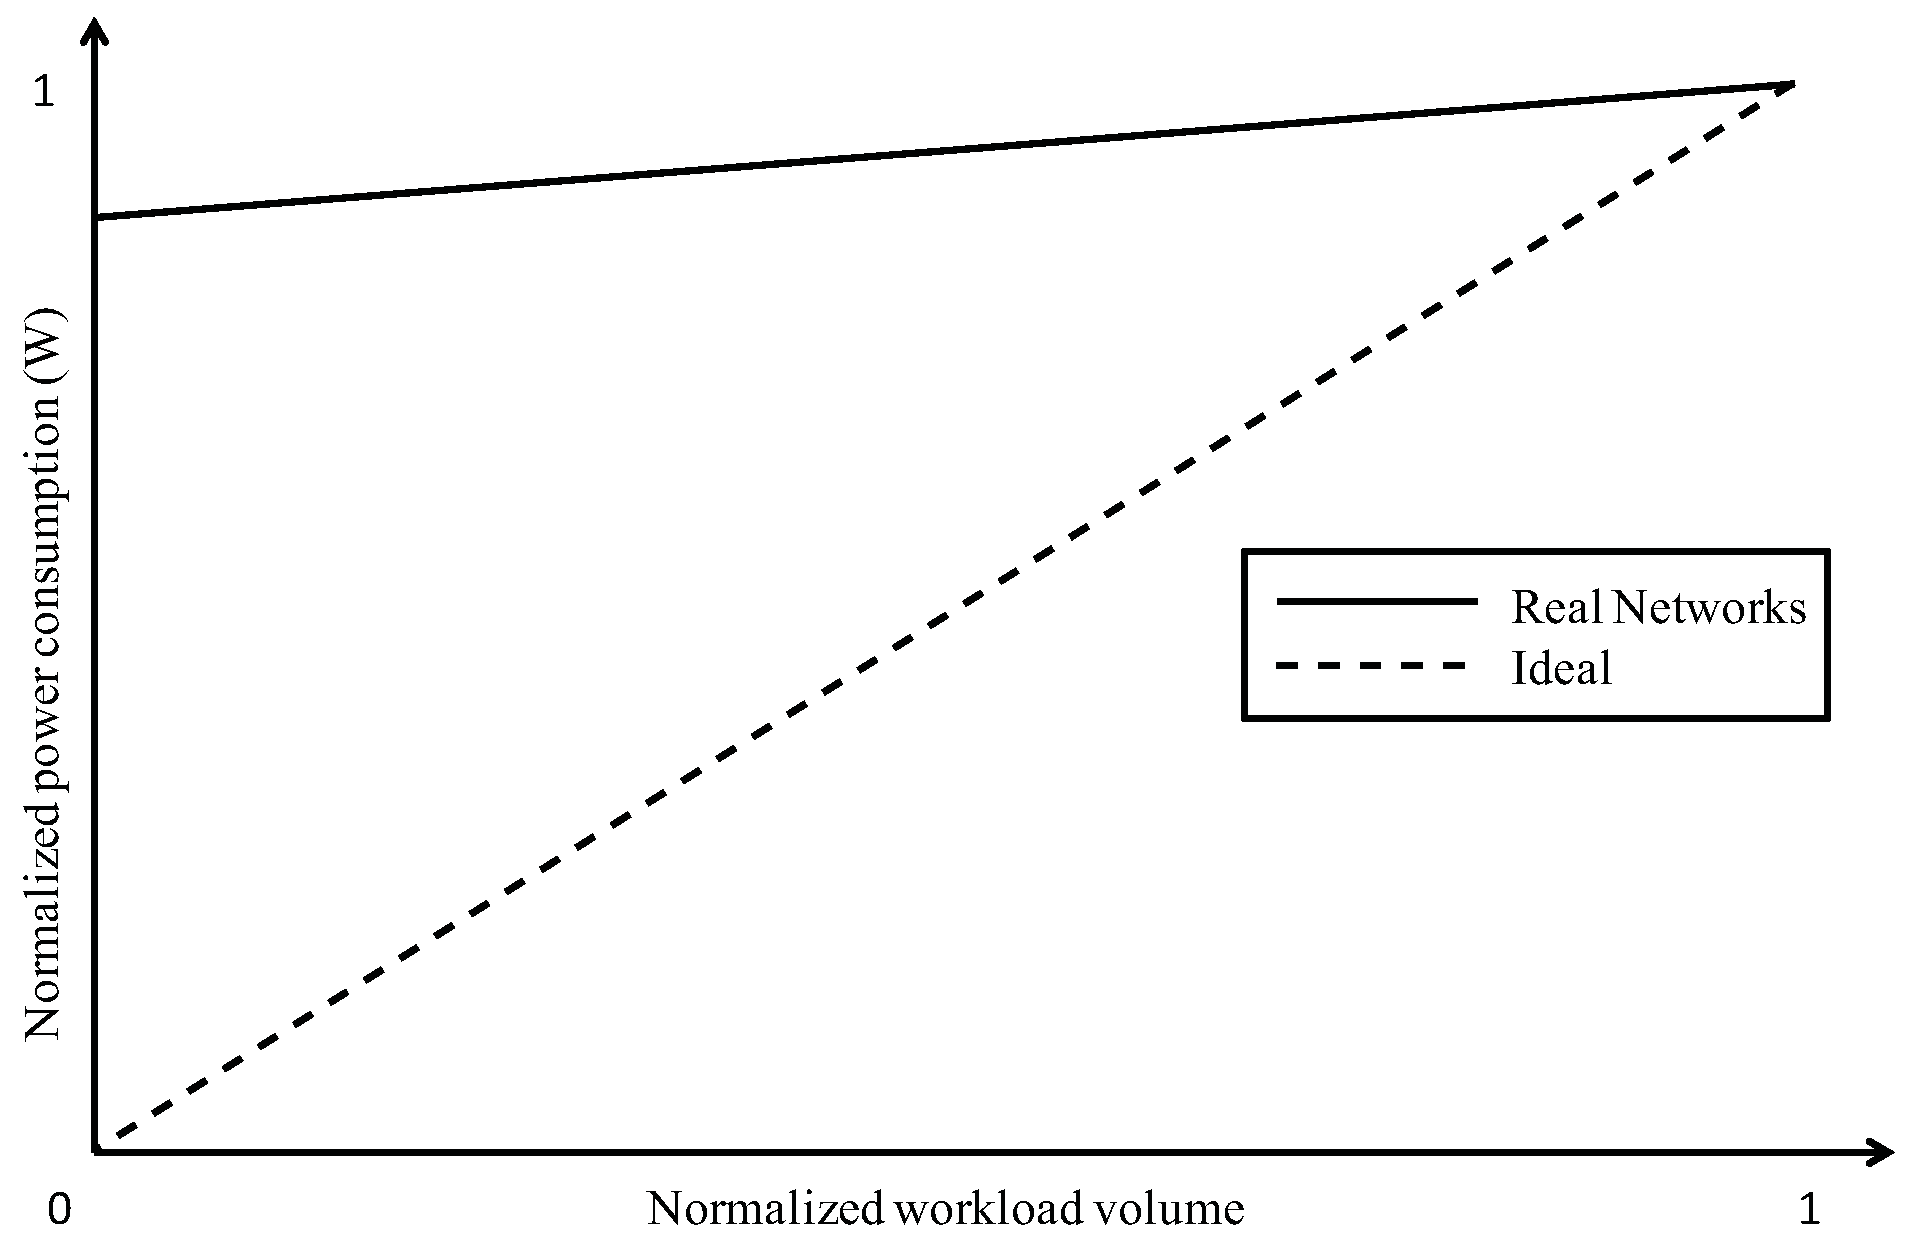
\includegraphics[width=1\textwidth]{pics/enerprop.eps}
\caption{Networks lack energy proportionality}
\label{fig:ener-prop}
\end{figure} 

A network that is not energy proportional is energy inefficient (i.e., consumes a lot more energy than it should) in the low-workload regimes. It has been observed for many networks that workload is variable and periodic. Figure~\ref{fig:varwork} shows the workload for call traffic at a cellular site in a large operational GSM network in Pakistan. It shows that call traffic has diurnal cycles and that traffic peaks for only a short period of time during a day. Furthermore, the workload peak is quite high compared to the trough. ISP~\cite{1248656} and data center~\cite{10.1109/MC.2007.443} traffic also show similar trends. In order to meet peak expected workload amicably, networks are dimensioned according to the peak workload. Since the workload is far from the peak most of the time and networks are not energy proportional, most networks are energy inefficient. Recent years have witnessed significant research effort aimed at improving network energy efficiency in packet networks, cellular networks and geo-diverse data centers. Effectively, such research aims to lower the y-intercept of the red line in Figure~\ref{fig:ener-prop}. 

\begin{figure}
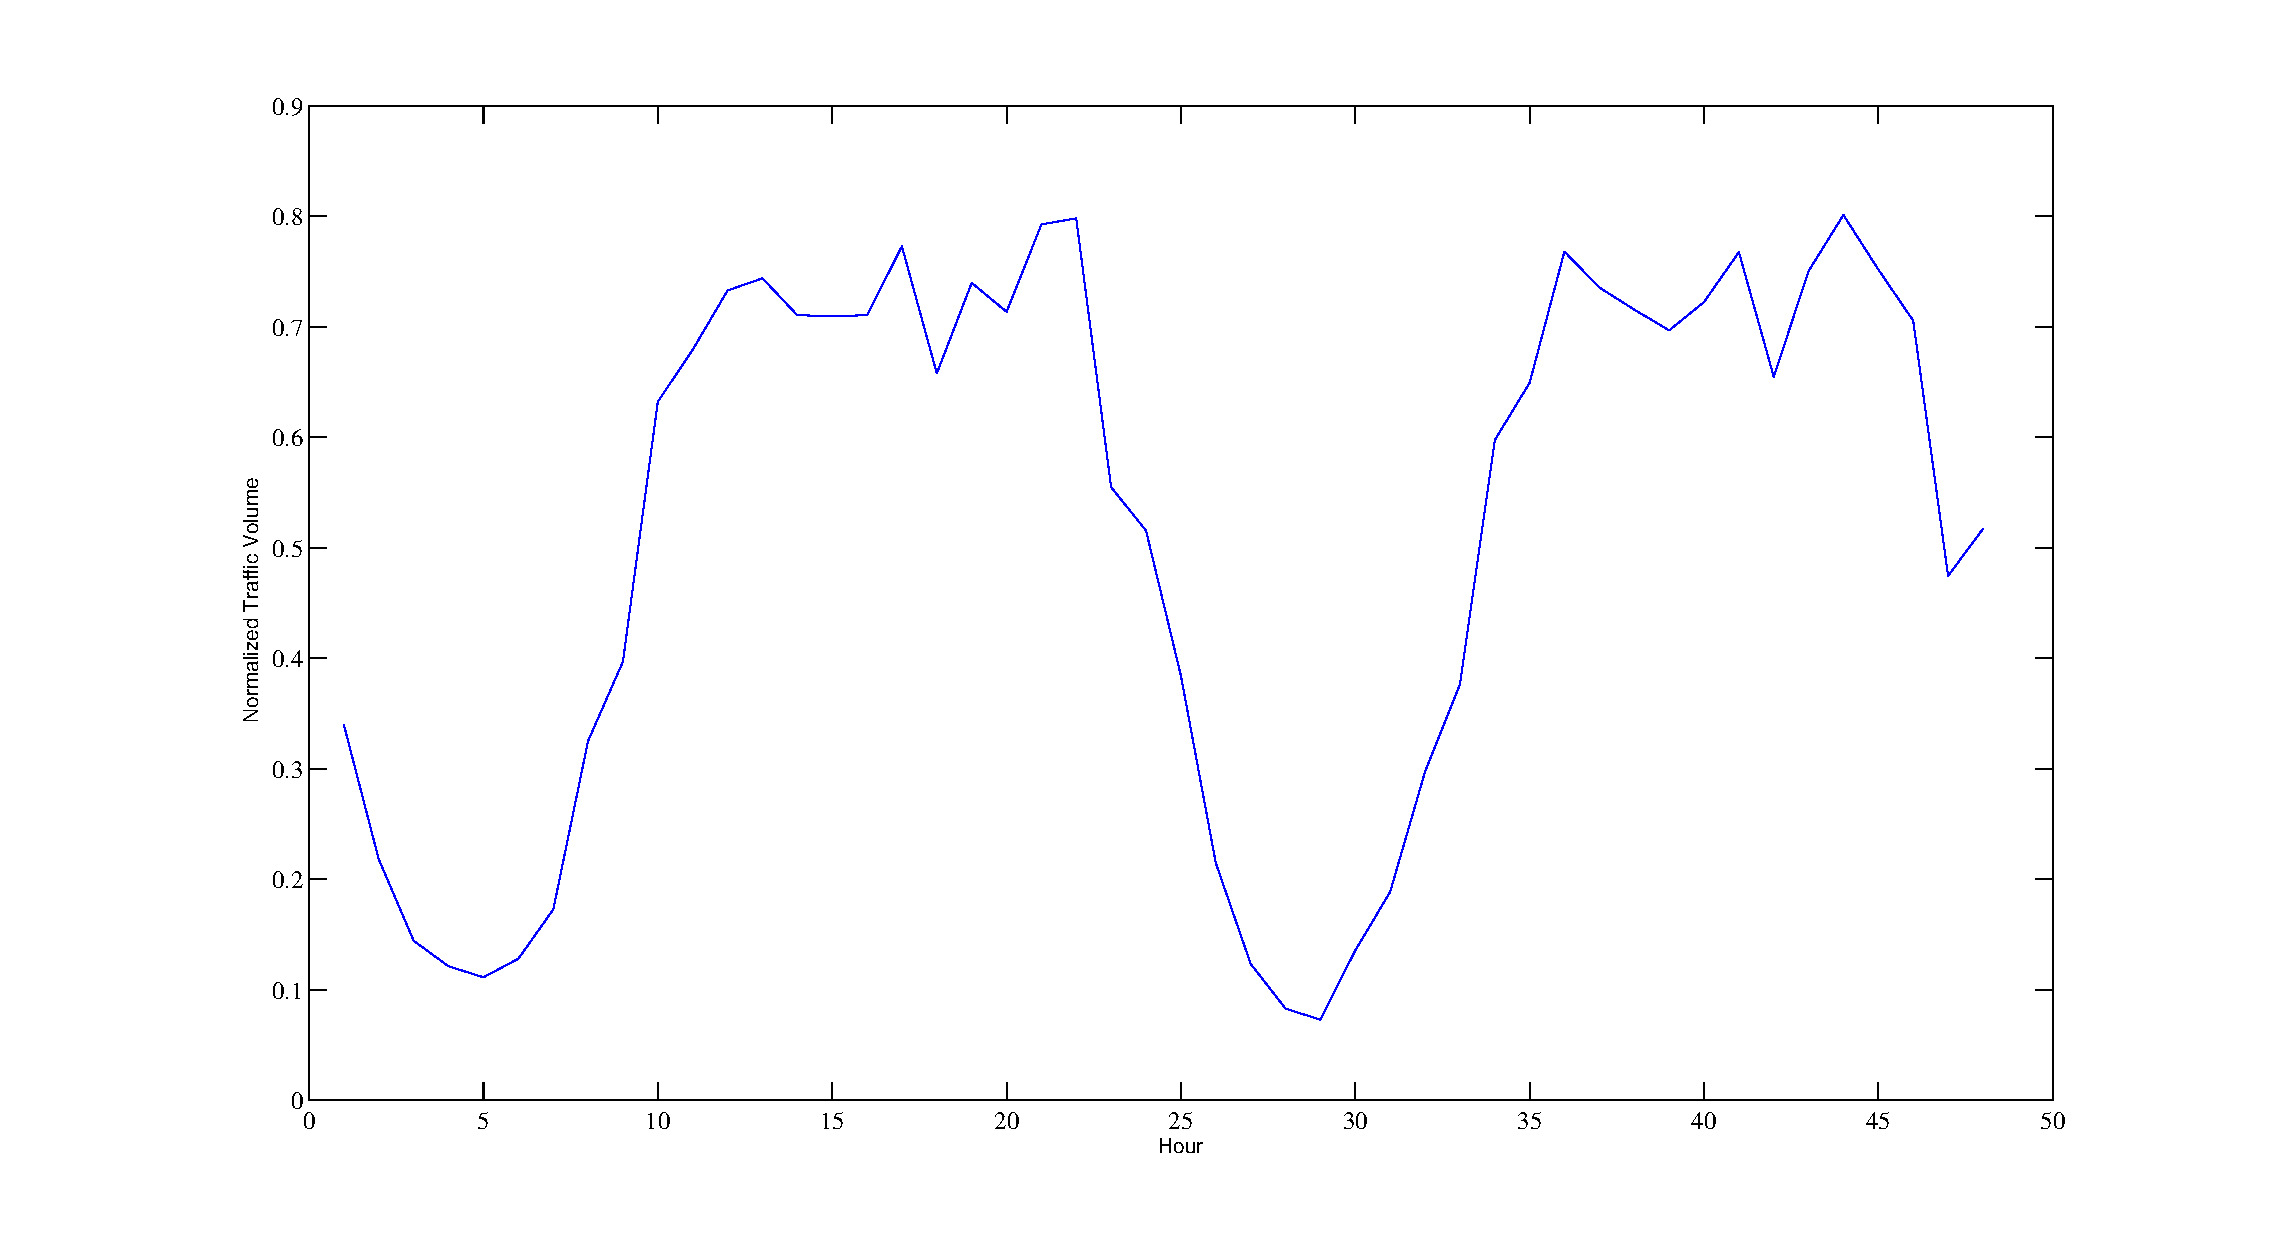
\includegraphics[width=1\textwidth]{pics/waridworkload.eps}
\caption{Call traffic for an oeprational cellular site over two days}
\label{fig:varwork}
\end{figure} 

We have observed earlier that network electricity costs are quite high. An energy efficient network would only incur high electricity costs if it handled a lot of workload. On the other hand, for energy inefficient networks, such as those prevalent today, high electricity costs are not justifiable by high workload because the workload is quite variable. In other words, today's networks have very poor performance per Watt characteristics. Therefore, reducing the electricity costs in today's networks is critically important.  


\section{Prevalent electricity cost reduction techniques} %\textit{Electricity cost} = \textit{amount of energy consumed} $\times$ \textit{unit price of electricity}. Therefore, electricity cost may be cut by reducing either or both of the quantities on the right hand side. 

The electricity cost for a network during a unit duration of time is given by:
\begin{align}
\text{Electricity cost} = \text{amount of energy consumed} \times \text{unit price of electricity}
\label{eq:elec-cost}
\end{align}
Conseuqently, the electricity cost for a network may be reduced by minimizing either or both of the terms on the right handside of the above equation. From prior research work and current operational practices in different types of networks, we observe the following techniques to reduce electricity cost in networks by reducing one or both of the two quantities in equation~\ref{eq:elec-cost}.

\subsection{Reducing the amount of energy consumed}
\begin{enumerate}
\item \textbf{Hardware upgrades:} Due to ecological challenges, improved energy efficiency is generally a key requirement when developing new technologies and devices. For a given workload demand, an improvement in device energy efficiency lowers the amount of energy consumed, thereby reducing electricity cost. Therefore, hardware upgrades are a way to reduce electricity costs. An operator would, however, opt for hardware upgrades in their network only after they have obtained the Return on Ivestment (ROI) of the initial deployment. The initial investment not only involves capital cost of equipment but other factors such as spectrum licensing as well. In the cut-throat competition prevalent in most of today's networks, the ROI is slow to achieve. This means that existing energy efficient networks would stay that way for a considerable tiem into the future.
\item \textbf{Hardware virtualization:} With the advent of ever faster CPUs, it was observed that servers tend to operate at relatively low CPU utilization most of the time. This was seen as an opportunity to statistically multiplex multiple servers onto a single physical machine by slicing the latter into multiple virtual servers. In this way, virtualization cuts capital costs for procurement of hardware. Since the virtual servers share the same resources (power supply, CPU, network interface, disks), if two servers are multiplexed onto a single physical server, the electricity consumption may be cut by as much as 50\%. A more aggressive server consolidation may cut electricity costs by upto 80\%~\cite{VirtualizationCutsPower}.
\item \textbf{Resource Pruning (RP):}Since network resources must be deployed according to peak demand while the workload peaks only for a short period of time, the excess resource may be deactivated (shutdown or put in power-saving mode depending on what is supported by the equipment) when workload is low~\cite{Chase:2001:MES:502059.502045,Chen:2008:ESP:1387589.1387613,Meisner:2009:PES:1508244.1508269,Lin_dynamicright-sizing,Peng:2011:TPS:2030613.2030628}. When evaluating the reduction in electricity costs through resource pruning, it is imperative to consider any costs associated with activation and deactivation of network resources.
\end{enumerate}

\subsection{Using cheaper electricity - Workload Relocation (WR)}
Electricity prices exhibit geographic diversity~\cite{qureshiHotnets}, i.e., the price of electricity varies from one location to another. The variation in electricity price is generally noticeable only at large distances. For instance, the electricity price anywhere within a city is generally the same\footnote{With the exception of factors such as different tarriffs for domestic, commercial and industrial consumers}. Most networks span large enough distances for geographic diversity in electricity prices to be apparent. If the network workload is quite flexible in terms of where it is handled, then the workload originating at a location with high electricity price may be relocated to a different location that has lower electricity price, thereby cutting electricity cost. We call this technique Workload Relocation (WR). We observe that different networks have different levels of geo-flexibility in workload. In geo-diverse data centers, for instance, the workload is highly geo-flexible, i.e., a client's request may be handled close by or even hundreds of miles away. On the other hand, the workload in cellular networks has very low geo-flexibility, i.e., a call mus tbe handled at a cellular base station within a few hundred meters from the caller.

Electricity prices also exhibit temporal diversity~\cite{qureshiHotnets}, i.e., the relative order of electricity prices at different locations keeps changing. If a city in Kansas presently has chepaer electricity than one in Oklahoma, an hour later, the reverse may be true. This means that mapping of workload to locations must be periodically updated. The granularity of these updates depends on how frequently electricity prices change. Electricity markets exhibit price changes at two different time scales (15 minutes for real-time electricity prices and an hour for day-ahead prices). 



\section{Our thesis} Based on the similarity in workload characteristics and the dependence of power consumption on workload, we opine that a generalized power optimization framework may be formulated that is applicable to many different types of networks. Our generalized electricity cost optimization framework would use workload relocation and resource pruning in tandem to reduce electricity costs\footnote{Hardware virtualization is complimentary to our framework}. 

\section{Contributions} This thesis makes the following contributions:

\begin{itemize}
\item We present a generalized model for electricity cost optimization applicable to different types of networks that jointly uses workload relocation and resource pruning. We show that this problem is NP-Hard.
\item We present a framework called Relocate Energy Demand to Better Locations (RED-BL), pronounced Red Bull, that solves this problem. We apply RED-BL to geo-diverse data centers as well as cellular networks using real data traces.
\item We exactly solve some reasonably-sized instances of this problem using real data. We also propose some heuristics that would be useful for larger instances of the problem. 
\item We evaluate RED-BL on two different types of networks, namely, geo-diverse data centers and cellular networks.
\item Prior efforts in this area had mostly ignored the costs associated with activation and deactivation of network resources. To the best of our knowledge, we are the first to incorporate these in our optimization framework.
\item We evaluate the benefits of geographical diversity exhibited by electricity prices and network deployments.
\item A network with significant overprovisioning may handle most of the workload at cheaper locations while the more expensive ones may be pruned from the network. In other words, geographic diversity in electricity prices incentivises over-provisioning. We study the benefits of increased over-provisioning and find diminishing returns when increasing over-provisioning.
\end{itemize}

\section{Organization} The rest of the document is structured as follows. In Chapter~\ref{chap:background}, we compare two different types of networks and describe how similar they are in terms of workload handling and power consumption. In chapter~\ref{chap:framework}, we derive a generalized power consumption model, applicable to different types of networks and formulate RED-BL, a generalized electricity cost optimization problem. We present an evaluation of RED-BL on geo-diverse data centers and cellular networks in chapters~\ref{chap:casestudy1} and~\ref{chap:casestudy2}, respectively. In chapter~\ref{chap:conclusions}, we draw the conslusions about our thesis and provide some future directions.